% 幂函数(复数)
% 复数|幂函数|反函数

我们先来看实参数的幂函数 $f(x) = x^a$, $x > 0$ 时函数曲线如\autoref{CPow_fig1} 所示. 注意 $x^{1/a}$ 是 $x^a$ 的反函数.
\begin{figure}[ht]
\centering
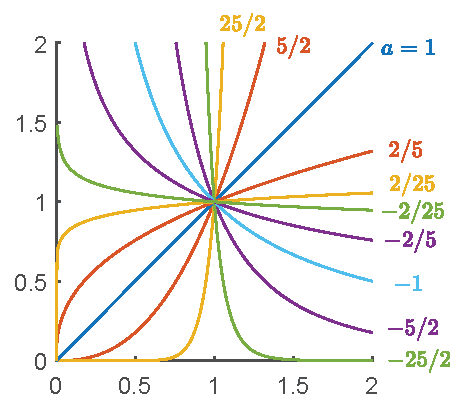
\includegraphics[width=8cm]{./figures/CPow1.pdf}
\caption{实参数的幂函数(相同颜色的函数互为反函数)} \label{CPow_fig1}
\end{figure}

当 $x < 0$ 时, 可得
\begin{equation}
x^a = \abs{x}^a (-1)^a = \abs{x}^a\E^{\I\pi a}
\end{equation}
当 $a$ 为偶整数时, $x^a = (-x)^a$ 是偶函数, $a$ 为奇整数时, $x^a = -(-x)^a$ 是奇函数. 当 $a$ 为非整数时, $x^a$ 必为复数, 其模长仍为$\abs{x}^a$, 幅角为常数 $\E^{\I\pi a}$.

\subsection{复参数的幂函数}
我们再来将复数的幂函数分解为模长和相位的形式(令 $z = \abs{z} \E^{\I\phi(z)}$, $a = a_I + \I a_R$ )
\begin{equation}
z^a = \abs{z}^{a_R} \E^{-\phi(z) a_I} \E^{\I[\ln\abs{z}a_I + \phi(z)a_R]}
\end{equation}
可见 $z^a$ 的模长和幅角都分别与 $z$ 和 $a$ 有关. 一般情况下, 这是一个比较复杂的函数, 含有不同的分支(因为 $\phi(z)$ 可以加整数个 $2\pi$).% 未完成: 分支是什么?
当且仅当 $a$ 为整数时才不会出现分支. 在数值计算中, 分支切割线出现在 $\phi(z) = \pm\pi$ 处, 这是因为数值计算通常取 $\phi(z)\in(-\pi, \pi]$.
